\documentclass[a4paper]{article}
\usepackage[latin1]{inputenc}
\usepackage{geometry}
\usepackage{amssymb}
\usepackage{framed}
\usepackage{amsmath}
\usepackage{graphicx}
\usepackage{booktabs}
\usepackage{subcaption}

\setlength{\parindent}{0pt}
\setlength{\parskip}{3ex}

\begin{document}

\begin{center}
  {\large Artificial Neural Networks and Deep Architectures, DD2437}\\
  \vspace{7mm}
  {\huge Short report on lab assignment 3\\[1ex]}
  {\Large Hopfield networks}\\
  \vspace{8mm}  
  {\Large Hilding Wollbo\\}
  \vspace{4mm}
  {\large September 27, 2020\\}
\end{center}

%\begin{framed}
%Please be aware of the constraints for this document. The main intention here is that you learn how to select and organise the most relevant information into a concise and coherent report. The upper limit for the number of pages is 6 with fonts and margins comparable to those in this template and no appendices are allowed. \\
%These short reports should be submitted to Canvas by the authors as a team before the lab presentation is made. To claim bonus points the authors should uploaded their short report a day before the bonus point deadline. The report can serve as a support for your lab presentation, though you may put emphasis on different aspects in your oral demonstration in the lab.
%Below you find some extra instructions in italics. Please remove them and use normal font for your text.
%\end{framed}

\section{Main objectives and scope of the assignment}
The tasks in the assignment concerned the study of auto-associative networks. In particular, Hopfield networks were implemented with different learning methods and studied for stability and storage capacity. The networks were also studied with regard to energy and distortion resistance.
\section{Results and discussion}
The tasks were implemented in Python using numpy and pandas for data manipulation while matplotlib was used to produce the graphics in the report.
\subsection{Convergence and attractors}
A Hopfield network was trained for the input patterns
\begin{align*}
  x_1 =& [-1, -1, 1, -1, 1, -1, -1, 1] \\
  x_2 =& [-1, -1, -1, -1, -1, 1, -1, -1] \\
  x_3 =& [-1, 1, 1, -1, -1, 1, -1, 1] \\
\end{align*}
using the synchronous Hebbian learning rule. That is, using the $N$ patterns in the input, the network weights were calculated as 
\begin{align*}
  \hat{W}_{k} =& W_k + \sum_{i=1}^N \mathbf{x_i} \mathbf{x_i}^T \\
  W_{k+1} =& \frac{1}{N} \hat{W}_{k} - \mathbf{I}.
\end{align*}
Convergence is reached when all patterns in the training set are mapped to themselves, i.e. $\mathbf{x} = W\mathbf{x}$. These points thus form \textit{attractors} in this network.
This network can also be used for reconstructing distorted versions of the original input patterns. The distorted test patterns
\begin{align*}
  x_{1d} =& [1, -1, 1, -1, 1, -1, -1, 1] \\
  x_{2d} =& [1, 1, -1, -1, -1, 1, -1, -1] \\
  x_{3d} =& [1, 1, 1, -1, 1, 1, -1, 1] \\
\end{align*}
were fed to the network. The first pattern contained a one-bit error and converged to $x_1$. The second and third patterns contained two bits error and were not mapped to one of the input patterns in the network. Instead, $x_{2d}$ was mapped to $[1, 1, -1, -1, -1, 1, -1, -1]$ and  $x_{3d}$ was mapped to $[-1, -1,  1, -1,  1,  1, -1, 1]$. Running these vectors through the weight matrix showed that they were mapped to themselves, thus also forming attractors for this network. Furthermore, when studying the network for attractors, the inverse of every training pattern is also a network attractor. Further spurious patterns can be found through linear ($\pm$) combinations of the input patterns.
The same architecture was also implemented for a larger dataset, an image dataset of 1024 pixels (weights) per image. A Hopfield network was trained for three images, shown in Figure $\ref{fig:training}$. This Hopfield network was then fed corrupted images of the input patterns, and the resulting output is shown in Figure $\ref{fig:reconstruction}$.
\begin{figure}[ht]
   \centering
   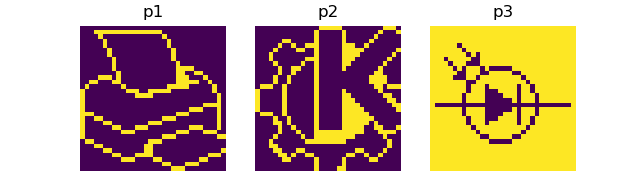
\includegraphics[width=\linewidth]{figures/training.png}
   \caption{The three training patterns}
   \label{fig:training}
\end{figure}
\begin{figure}[ht]
   \begin{subfigure}[b]{0.5\textwidth}
   \centering
   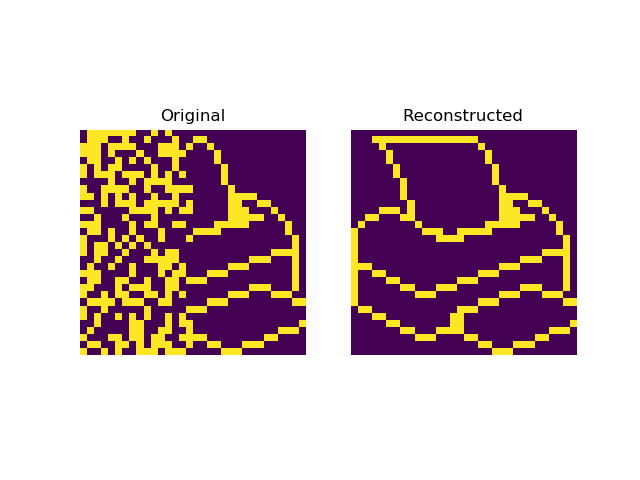
\includegraphics[width=\linewidth]{figures/p10b.png}
   \subcaption{The reconstruction of the corrupted pattern p10}
   \end{subfigure}
  \begin{subfigure}[b]{0.5\textwidth}
   \centering
   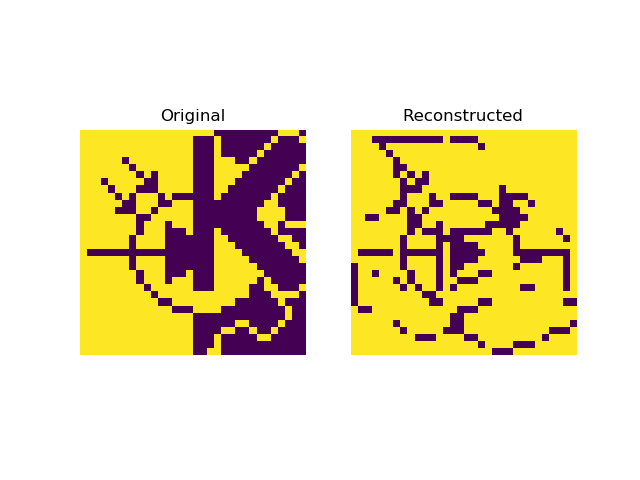
\includegraphics[width=\linewidth]{figures/p11b.png}
   \subcaption{The reconstruction of the corrupted pattern p11}
   \end{subfigure}
   \caption{Reconstruction using the Hopfield network}
   \label{fig:reconstruction}
\end{figure}
% Image with p10, p10 after batch, p11, p11 after batch
\subsection{Sequential Update}
In the original Hopfield network, however, the update for the input data is not synchronous, i.e. all output nodes are not updated at the same time. By updating one output node at a time, the updated node can influence the outcome of subsequent nodes in the same epoch. This asynchronous update rule was implemented for the two corrupted patterns, leading to the convergence shown in Figure \ref{fig:asynchronous}. The initial energy values of the different patterns is shown in Table \ref{tab:energy}.
\begin{table}
\centering
\begin{tabular}{@{}llllll@{}}
  \toprule
    Image & p1 & p2 & p3 & p10 & p11 \\
  \midrule
    Energy & -1438 & -1364 & -1461 & -414 & -171 \\
\bottomrule
\end{tabular}
\caption{The initial energy of the different patterns.}
\label{tab:energy}
\end{table}
\begin{figure}[ht]
   \begin{subfigure}[b]{0.5\textwidth}
   \centering
   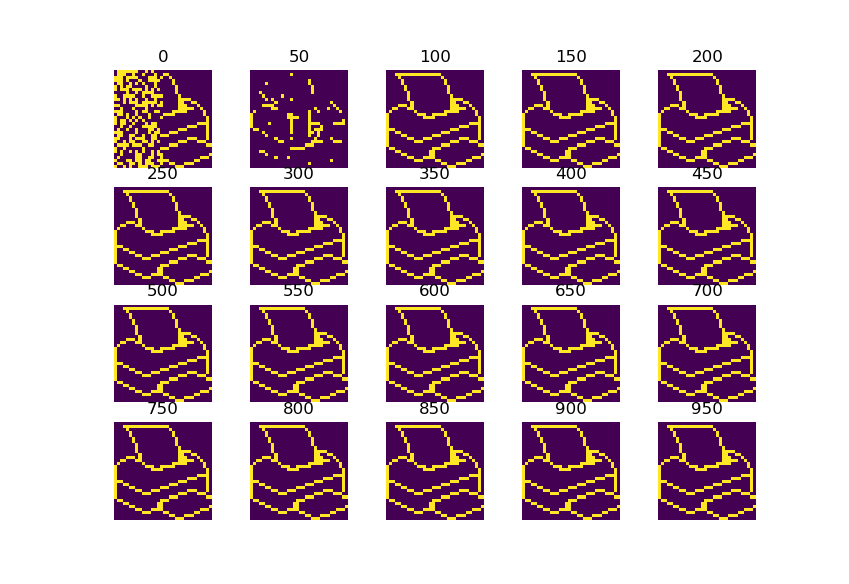
\includegraphics[width=\linewidth]{figures/p10.png}
   \subcaption{The reconstruction of the corrupted pattern p10}
   \end{subfigure}
  \begin{subfigure}[b]{0.5\textwidth}
   \centering
   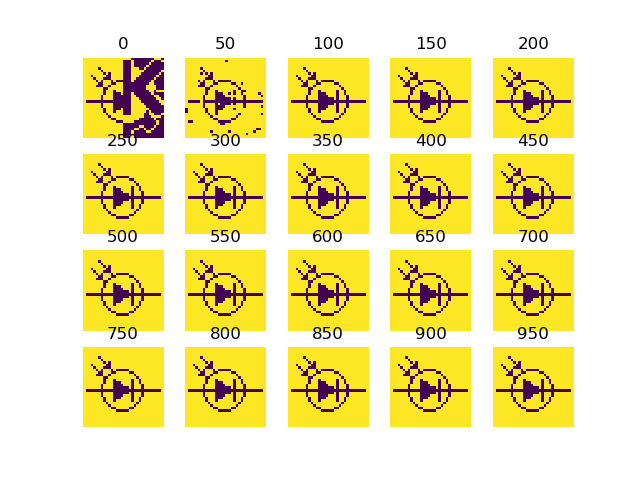
\includegraphics[width=\linewidth]{figures/p11correct.png}
   \subcaption{The reconstruction of the corrupted pattern p11}
   \end{subfigure}
   \caption{Reconstruction using the Hopfield network with asynchronous update}
   \label{fig:asynchronous}
\end{figure}
% Image with p10 during sequential, image with p11 during sequential
\subsection{Energy}
One way to measure the progess of the network during output update is to measure the energy of the network as the update progresses. There are many possible measures, but one simple is given by the Lyapunov function 
\begin{align*}
  E = - \mathbf{x}^T W \mathbf{x}
\end{align*}
It should be noted that a proper Hopfield matrix $W$ simply transforms the alignment of the input vectors and does not add any energy. The patterns p0, p1 and p2 all directly map to themselves, and the energy is constant. The corrupted patterns p10 and p11 eventually map to a constant pattern, as was seen in Figure \ref{fig:asynchronous}.
The energy of the two patterns as the update progresses is shown in Figure \ref{fig:energy}.
 \begin{figure}[ht]
   \begin{subfigure}[b]{0.5\textwidth}
   \centering
   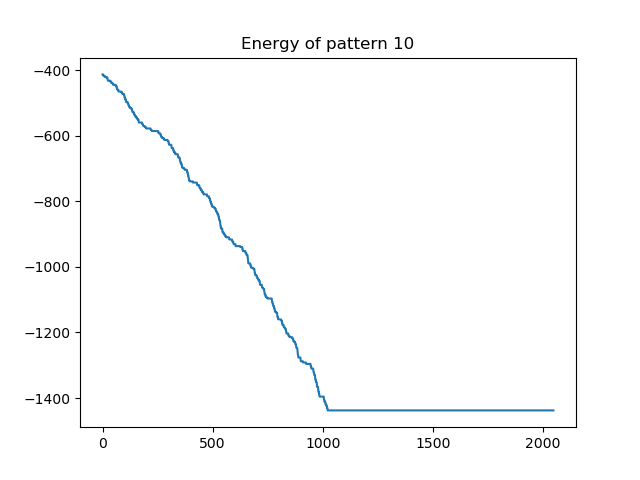
\includegraphics[width=\linewidth]{figures/ep10.png}
   \subcaption{The energy of the corrupted pattern p10}
   \end{subfigure}
  \begin{subfigure}[b]{0.5\textwidth}
   \centering
   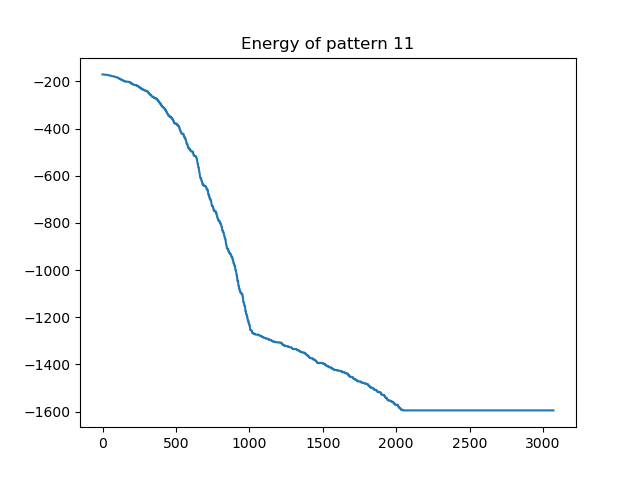
\includegraphics[width=\linewidth]{figures/ep11.png}
   \subcaption{The energy of the corrupted pattern p11}
   \end{subfigure}
   \caption{Energy using the Hopfield network with asynchronous update}
   \label{fig:energy}
\end{figure}
We could compare this to the performance of random initialization as well. The weight matrix was initialized as a completely random normal gaussian variable, which resulted in the energy convergence in Figure \ref{fig:energyrandom}. With this initialization, the initial energy is a lot higher since the matrix isn't normalized. The energy converges to a lower energy range where it oscillates.
\begin{figure}[ht]
   \begin{subfigure}[b]{0.5\textwidth}
   \centering
   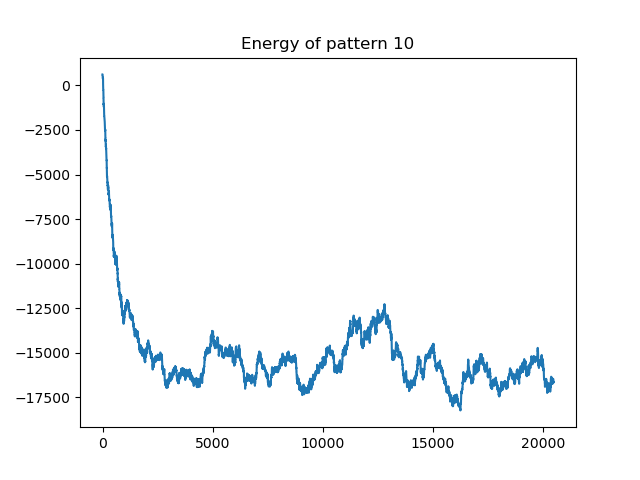
\includegraphics[width=\linewidth]{figures/ep10r.png}
   \subcaption{The energy of the corrupted pattern p10}
   \end{subfigure}
  \begin{subfigure}[b]{0.5\textwidth}
   \centering
   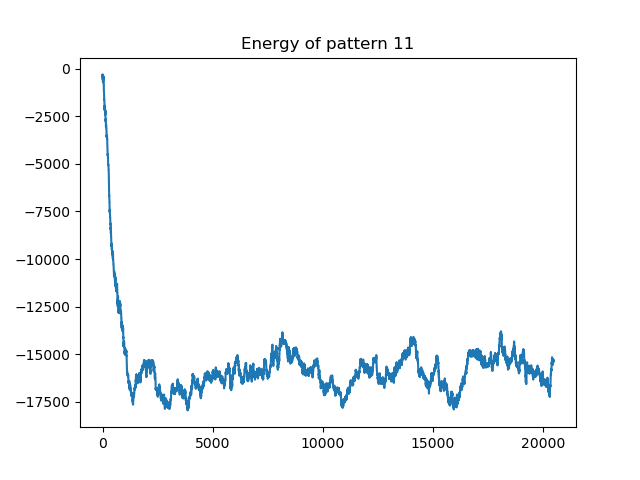
\includegraphics[width=\linewidth]{figures/ep11r.png}
   \subcaption{The energy of the corrupted pattern p11}
   \end{subfigure}
   \caption{Energy using the Hopfield network with random weight matrix}
   \label{fig:energyrandom}
\end{figure}
We could also compare with a random by symmetrical matrix, with proper zero diagonal. Using this initialization yielded the energy curve in Figure \ref{fig:energysymmetric}. This energy curve is a lot more well behaved. This is because in its symmetrical nature, the connections from an output node is also affected when its input weights are changed, leading to a much faster convergence.
\begin{figure}[ht]
   \begin{subfigure}[b]{0.5\textwidth}
   \centering
   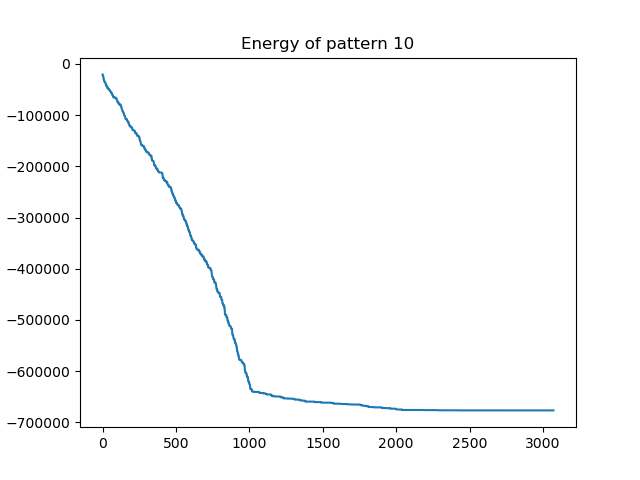
\includegraphics[width=\linewidth]{figures/ep10s.png}
   \subcaption{The energy of the corrupted pattern p10}
   \end{subfigure}
  \begin{subfigure}[b]{0.5\textwidth}
   \centering
   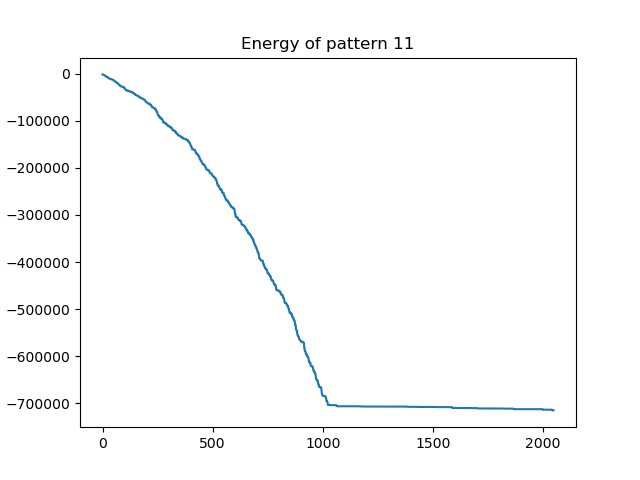
\includegraphics[width=\linewidth]{figures/ep11s.png}
   \subcaption{The energy of the corrupted pattern p11}
   \end{subfigure}
   \caption{Energy using the Hopfield network with symmetrical weight matrix}
   \label{fig:energysymmetric}
\end{figure}
\subsection{Distortion Resistance}
The Hopfield network is also known for its resistance to distortion, since it is an autoassociative memory. Therefore, to study the noise resistance, the three training patterns were manipulated with various amounts of bits flipped and subsequently fed to a trained Hopfield network. The network was able to correct for atleast 30 \% of bits flipped, shown in Figures \ref{fig:dist1}, \ref{fig:dist2} and \ref{fig:dist3}. After reaching more than half of the bits flipped, the network mapped the input to its symmetrical, inverted spurious pattern.
\begin{figure}[ht]
   \centering
   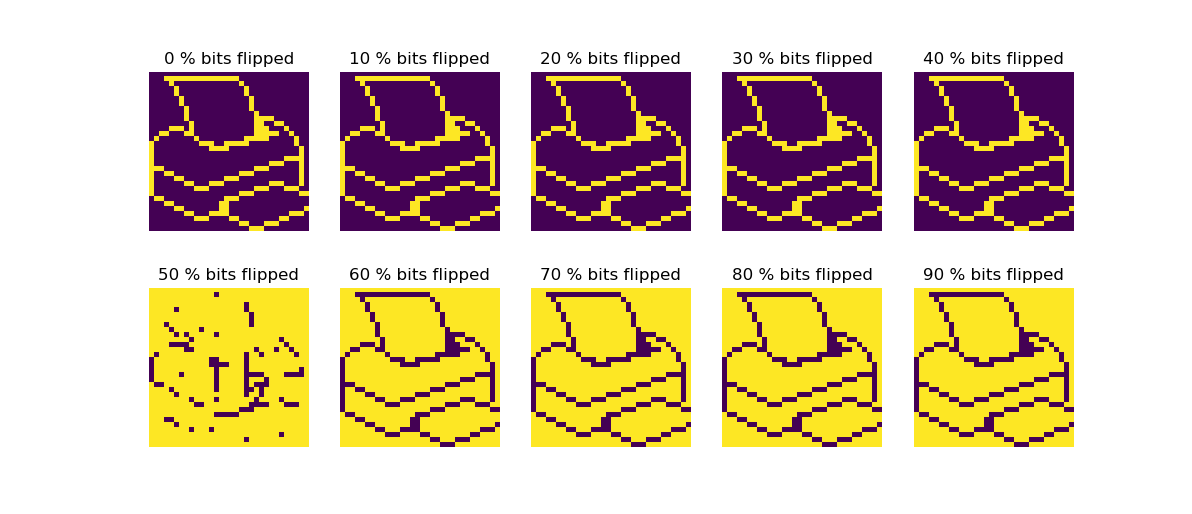
\includegraphics[width=\linewidth]{figures/d1.png}
   \caption{Output of the first pattern after distortion}
   \label{fig:dist1}
\end{figure}
\begin{figure}[ht]
   \centering
   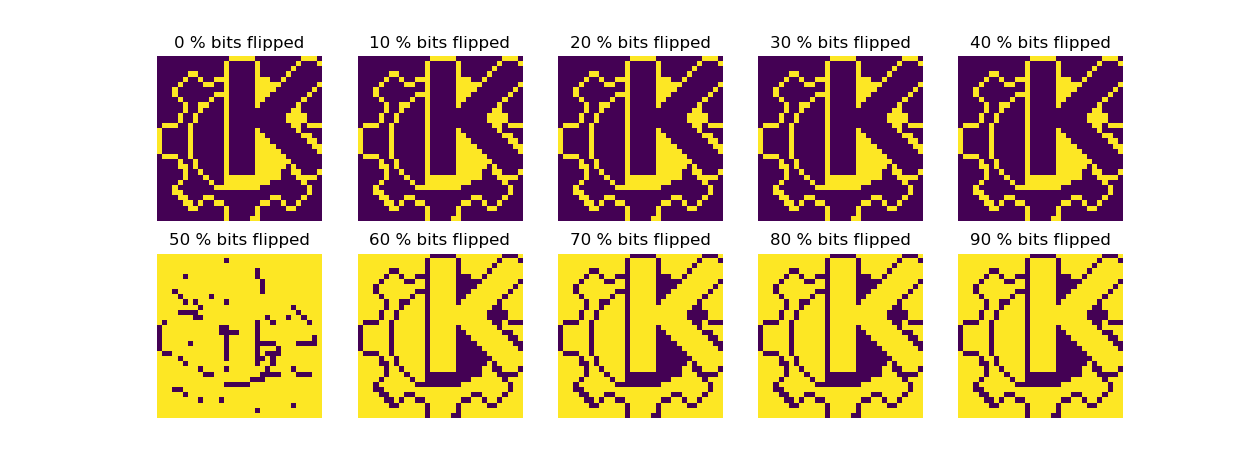
\includegraphics[width=\linewidth]{figures/d2.png}
   \caption{Output of the second pattern after distortion}
   \label{fig:dist2}
\end{figure}
\begin{figure}[ht]
   \centering
   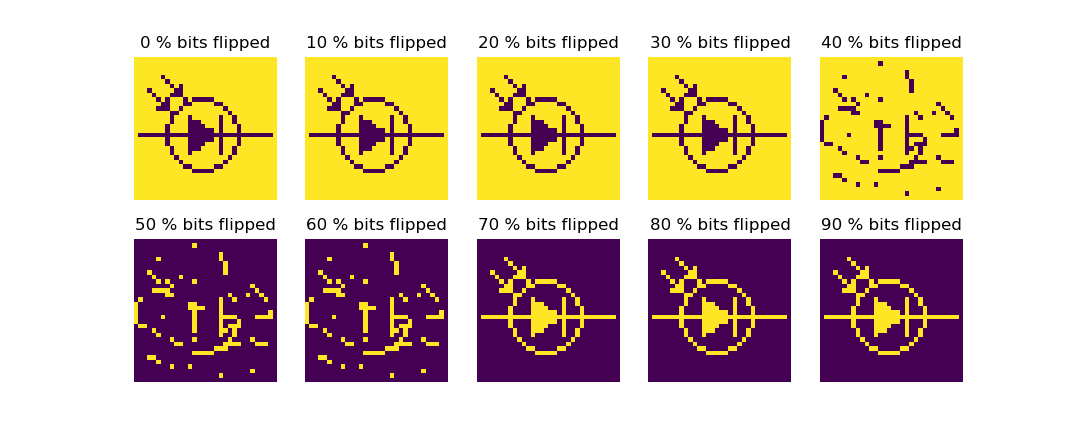
\includegraphics[width=\linewidth]{figures/d3.png}
   \caption{Output of the third pattern after distortion}
   \label{fig:dist3}
\end{figure}
\subsection{Capacity}
Previously, we had only used three different patterns to train on and store. One interesting aspect of Hopfield networks is their capacity to store different patterns. However, by just increasing the number of training patterns to four immediately made the network unable to reconstruct any of the input patterns to their original. This is because the network already learns many spurious patterns, and also because the images are not orthogonal (i.e. correlated to some degree).
However, Hopfield networks have an alleged theoretical capacity of $0.138N$. By generating random uncorrelated patterns this capacity was investigated. The network was selected with size 150, and 300 different random patterns were generated for training. 
The proportion of correctly recalled patterns for this network was plotted when varying the number of training patterns in Figure \ref{fig:capa}. This network was on average able to store around 18 patterns, which is roughly the same as the theoretical limit of 20 patterns. The same network was investigated when adding 1 \% noise in the form of flipped bits. The performance for this scenario is shown in Figure \ref{fig:capb}.
\begin{figure}[ht]
   \begin{subfigure}[b]{0.5\textwidth}
   \centering
   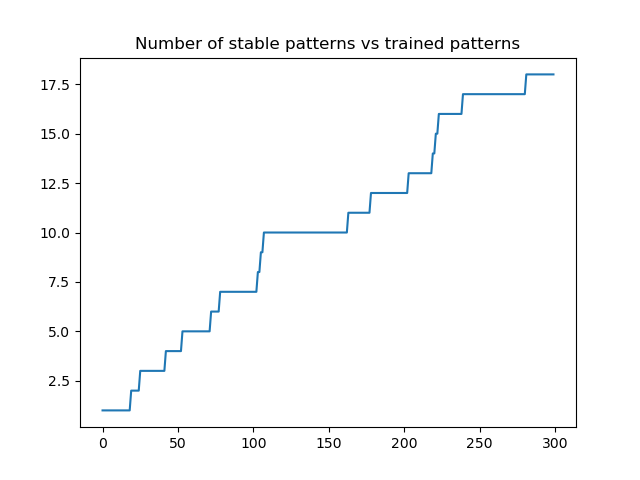
\includegraphics[width=\linewidth]{figures/c150.png}
   \subcaption{The capacity of the 150 node network.}
   \label{fig:capa}
   \end{subfigure}
  \begin{subfigure}[b]{0.5\textwidth}
   \centering
   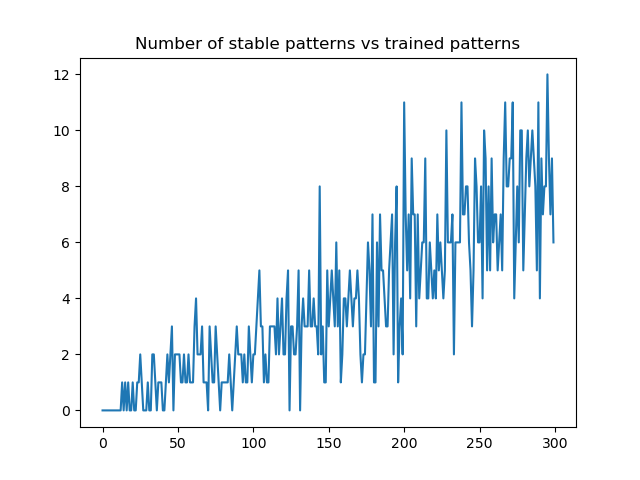
\includegraphics[width=\linewidth]{figures/c150n.png}
   \subcaption{The capacity of the 150 node network with 1 \% noise.}
   \label{fig:capb}
   \end{subfigure}
   \caption{The number of correctly recalled patterns as training progresses.}
   \label{fig:cap}
\end{figure}
It should be noted that the Hopfield network I implemented in earlier sections had zero self connections, i.e. $w_{ii} = 0 \ \forall \ i$. For this task and the patterns generated, however, it was necessary to add these self connections for almost anything to be correctly recalled. This is because the random patterns generated are essentially uncorrelated in each dimension, which causes the patterns to directly map to themselves when multiplied by the weight matrix. This also trivializes the Hopfield network, since all it essentially does is act as an identity matrix.
Removing the self-connections yielded vastly different results, where performance breaks down completely when adding more than 30 patterns to the weight matrix. Biasing the patterns lead to a drastic reduction in performance, and only a handful of patterns could be stored in the matrix. Similar to the case with the pictures, this is due to the bias of the patterns leading to more correlation between patterns, which increases the probability of confusing two patterns and an increase in the amount of errors.
\subsection{Sparse Patterns}
In order to solve the problems imposed by biased patterns, the training and update rules can be modified by adding an average activity term to the hebbian training rule and a bias term to the update rule. Generating sparse patterns (low amounts of ones) shows the importance of this bias term. The resulting maximal patterns stored as a function of the bias term is shown for three different sparsity levels in Figure \ref{fig:sparsity}. It can be seen that the peak shifts to the left as the patterns become more sparse. Thus, for more sparse patterns, it is better to use a lower bias.
\begin{figure}[ht]
  \begin{subfigure}[b]{0.3\textwidth}
   \centering
   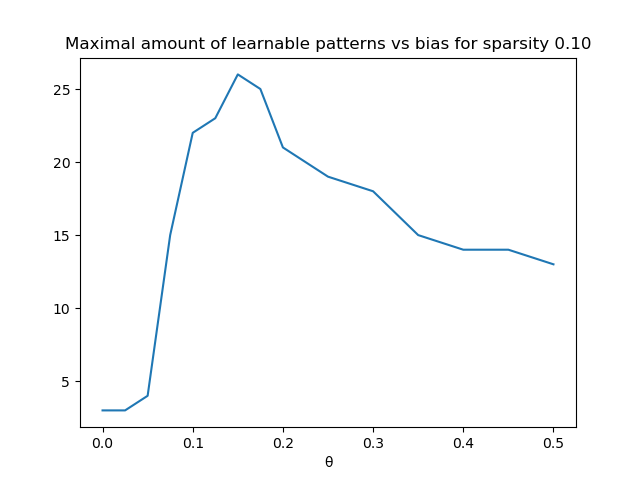
\includegraphics[width=\linewidth]{figures/c150s010.png}
   \subcaption{Sparsity 10 \%}
  \end{subfigure}
  \begin{subfigure}[b]{0.3\textwidth}
   \centering
   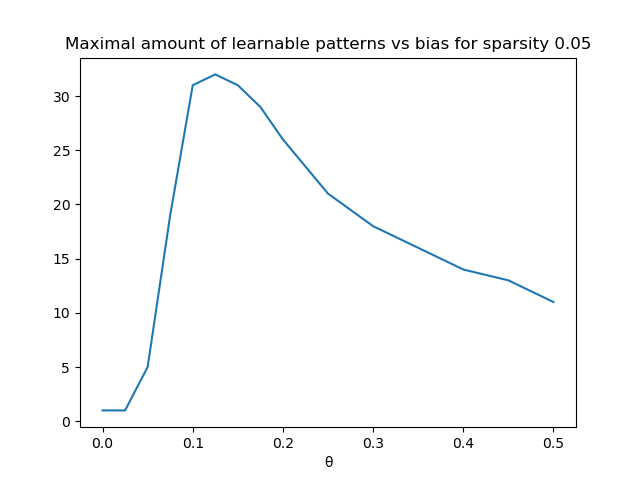
\includegraphics[width=\linewidth]{figures/c150s005.png}
   \subcaption{Sparsity 5 \%}
  \end{subfigure}
  \begin{subfigure}[b]{0.3\textwidth}
   \centering
   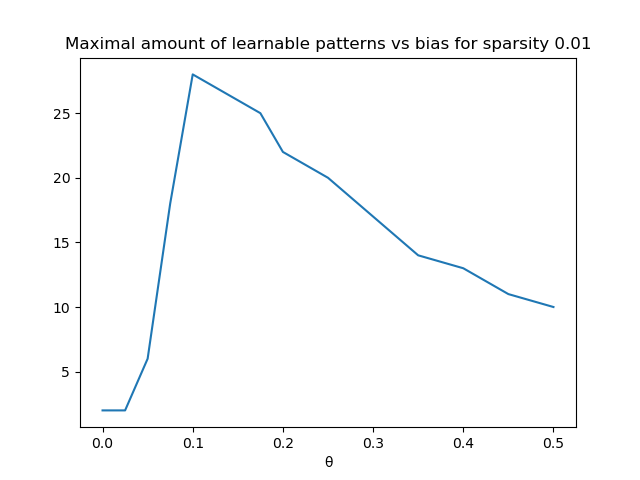
\includegraphics[width=\linewidth]{figures/c150s001.png}
   \subcaption{Sparsity 1 \%}
   \end{subfigure}
   \caption{The maximal amount of storable patterns as a function of the bias for different sparsity levels.}
   \label{fig:sparsity}
\end{figure}
\section{Final remarks }
This was an interesting lab, and it helped very much in order to understand the auto associative principles of the Hopfield network through implementing it from first principles. I do wish that there were more structured datasets for which to implement these tasks, since one of the major unexpected behaviours I found with the capacity task I attribute to the randomly generated data.
\end{document}